
\subsection{PIPP}
\label{sec:algorithms:pipp}

Promotion/Insertion Pseduo-Partitioning~\cite{Xie2009} (PIPP) proposed in 2009 is an algorithm based on a slightly modified UMON circuit and a novel insertion and promotion policy.
The UMON changes are to enable stream detection.
Where the UCP algorithm only handles streaming applications indirectly, by assigning few ways because of a low hit rate in the ATDs, PIPP's UMON actively detects streaming applications.
Stream detection is implemented by adding a counter that counts the total number of cache misses in the ATD.
An application is then deemed to be streaming if either the number of misses or the miss rate in a single allocation period is above a threshold.

PIPP like UCP views the cache set as an LRU stack.
The replacement policy is as in LRU, but the insertion and promotion policy is novel.
The insertion policy inserts new blocks $\pi_n$ blocks from the LRU position. 
Here $\pi_n$ is the number of ways assigned to the $n^{th}$ core.
In a 4-way cache dual-core setup where both cores are assigned two ways, PIPP will insert all new blocks from either core in the second to last position in the stack. 
In this situation, the two top positions in the cache stack can only be reached by a cache block through promotion.
On a cache access, a block has a chance, $p_{prom} = \frac{3}{4}$, to move one position upwards in the stack unless it is already at the MRU position.

On insertion, the PIPP policy does not consider how many blocks are owned by the requesting core, this is unlike UPC's insertion policy that prevents a core form claiming more ways that what it is assigned.
However, cores with more ways assigned to it will insert its blocks higher up in the stack. 
The core with the highest number of ways assigned will not have any insertion competition pushing its blocks out of the cache.
The only way blocks from this core can be pushed out is by other blocks from the same core, or by blocks from other cores that are re-referenced repeatably.
Two cores with the same allocations will both have an equal chance of keeping their blocks in the cache, as they both insert at the same position.
Statistically a core with a lower allocation, inserting at a lower position in the stack, should also on average own fewer blocks in the cache compared to a core with a higher allocation.
This way PIPP obtains what the original authors call pseudo partitioning, where overall a higher allocation will statistically result in more cache space.
However, the access frequency of cores can cause a core with a low allocation to own most of or all blocks in the cache if the other cores have a much lower access frequency.

When the UMON detects a core that is streaming PIPP will no longer insert blocks from this core at the position given by the allocation.
A special insertion position, $\pi_{stream}$, is used for all streaming cores.
$\pi_{stream}$ is set to the number of cores currently streaming. 
By inserting at this fixed position, PIPP attempts to limit the interference the streaming core has on the non-streaming cores.
Blocks from streaming applications have a reduced chance of promotion after an access, $p_{stream} = \frac{1}{128}$.
In the case where all cores are streaming, and there are no cores to protect, PIPP inserts all blocks at the LRU position.

Figure~\ref{fig:algorithms:pipp_example} shows an example cache set managed by PIPP shared by two cores.
Both cores are allocated two blocks, and initially core 0 owns three blocks in the set; A, C, and D.
In this example we assume all hits cause a block promotion.
The first request is for C by core 0; this is a hit, and the block is promoted, effectivly swapping block B and C.
Next is a request for E by core 0; this is a miss.
E is inserted at the second to last position of the cache set, as the core is allocated two blocks, causing D to be evicted and B to move to the LRU position.
Finally, a request for F is made by core 1; again it is inserted at the second to last position, evicting B.
Note that after the initial request for C, the state of the two upper blocks do not change.

\begin{figure}[ht]
    \centering
    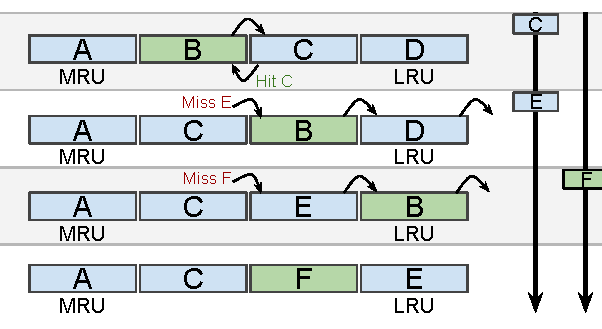
\includegraphics[width=.65\textwidth]{figures/algorithms/PIPP}
    \caption[PIPP managed 4-way cache set.]{PIPP managed 4-way cache set. (Two cores each allocated two blocks)}
    \label{fig:algorithms:pipp_example}
\end{figure}